\documentclass[a4paper,twoside]{article}

\usepackage{epsfig}
\usepackage{subfigure}
\usepackage{calc}
\usepackage{amssymb}
\usepackage{amstext}
\usepackage{amsmath}
\usepackage{amsthm}
\usepackage{multicol}
\usepackage{pslatex}
\usepackage{apalike}
\usepackage{graphicx}
\usepackage{algorithmic}
\usepackage{textcomp}
\usepackage{SCITEPRESS}     % Please add other packages that you may need BEFORE the SCITEPRESS.sty package.

\subfigtopskip=0pt
\subfigcapskip=0pt
\subfigbottomskip=0pt

\begin{document}

\title{Tiny Planets}

\author{\authorname{Sharzard Gustafson, Matthew Pohlmann, Ricardo Sisnett}
\affiliation{University of Southern California, Los Angeles, USA.}
\email{\{sagustaf, pohlmann, sisnetth\}@usc.edu}
}

\keywords{Procedural Generation, Graphics, Perlin Noise}

\abstract{ In this paper we present a method of procedurally generating stylized planetary models with geography by combining multi-fractal Perlin noise and recursive icospheres. Planets are further decorated with procedurally modeled vegetation placed accordingly to the geography. A materials system was implemented to visualize the results of the generation algorithms.}

\onecolumn \maketitle \normalsize \vfill

\section{\uppercase{Introduction}}
\label{sec:introduction}
\noindent In this work we present the results of implementing a series of techniques in a bare bones real-time graphics engine, extending its core by adding a materials system and creating an application that utilizes procedural modeling techniques to create planetoids with natural looking geographical features. The graphics engine is built using the Simple DirectMedia Layer (SDL), a cross-platform solution for access to low-level peripherals and graphics hardware, and the openGL Extension Wrangler library (GLEW).

\section{\uppercase{Material System}}
\label{sec:mat_sys}
\noindent A material system is a framework that builds on top of and abstracts the functionality and bindings of basic vertex and pixel/fragment shaders, and is commonly used in real-time graphics applications \cite{gengines}. Materials combine a vertex and fragment shader in order to re-use common shading functionality amongst multiple meshes, provide access to shader parameters (like emissive and diffuse colors, specular power, textures, etc.), and allow for custom math expressions in order to customize the appearance of different surfaces; the result is that only these parameters and expressions need to be changed to represent a multitude of surfaces rather than writing and loading shader programs for each surface. An added benefit is that it becomes possible to render all meshes with common materials without changing the shader program on the GPU by simply modifying the current shader program's inputs, thereby improving performance.
Our material system implements basic Phong shading in a single vertex and fragment shader pair, and allows customization of ambient, emissive, diffuse, and specular colors, specular power, and a single texture. The system also adopts the concept of material instances in order to allow different meshes using the same material to modify parameters without affecting each other. Figure \ref{fig_ms} is a visual representation of the system we have designed and implemented for the project. The quicker iteration time provided by the material system in customizing the different meshes in the application allowed us to focus on achieving the stylized look of our original goal.

\begin{figure}
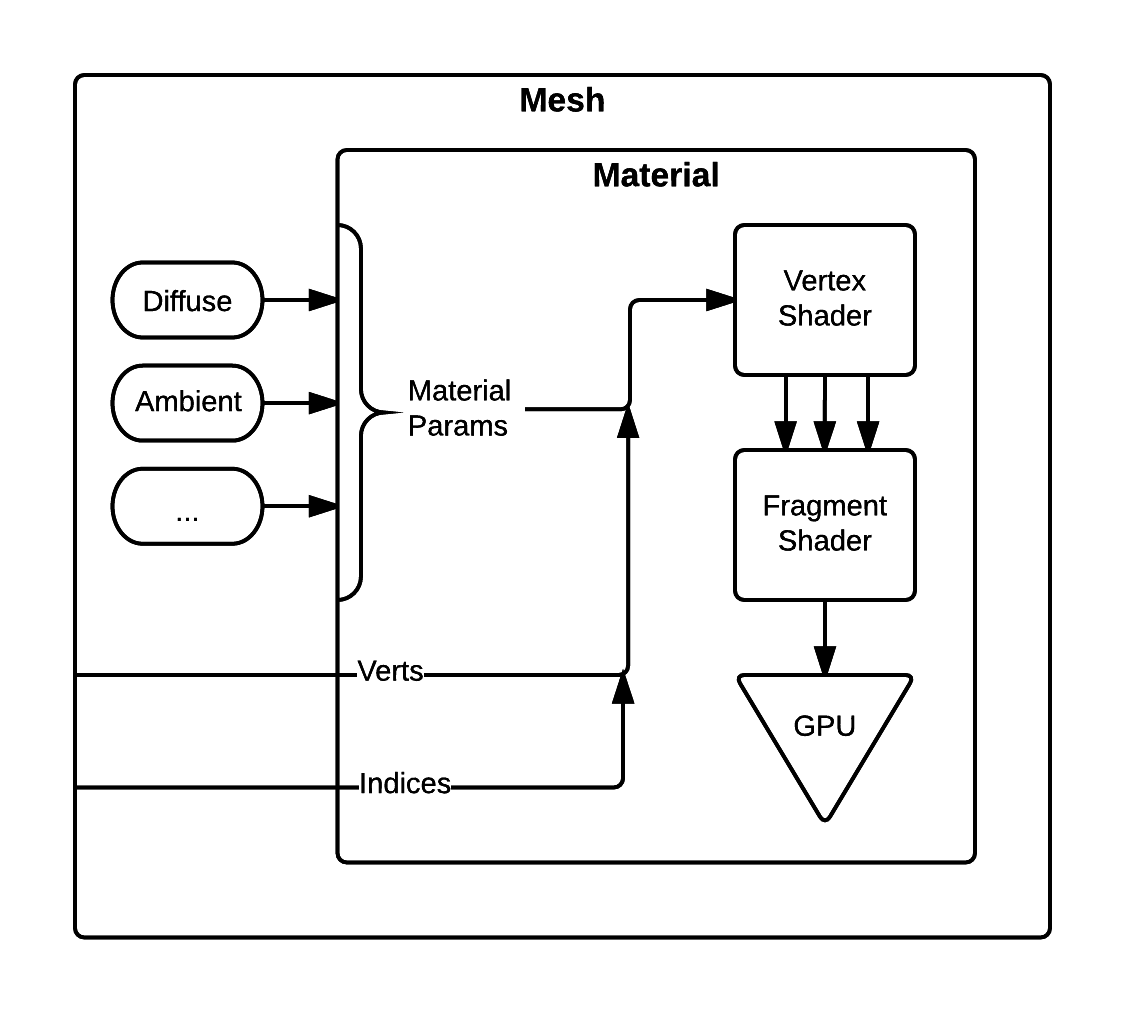
\includegraphics[scale=0.75]{./images/materials/ms_overview.png}
\caption{Technical diagram of our simple material system}
\label{fig_ms}
\end{figure}

\section{\uppercase{IcoSpheres}}
\label{sec:icosphere}
\noindent An icosphere is one of two of the most common ways of rendering spheres in computer graphics applications, the other being the UV sphere. An icosphere starts by taking a 20-sided polyhedron (icosahedron)  and recursively subdividing the faces to add detail. This method of generation causes the sphere's vertexes to be evenly distributed along the surface, which is a desirable trait for our use case as it lends itself better for deformation than UV spheres \cite{pnoise}. Figure \ref{fig_isa} illustrates the basic idea behind this algorithm. The number of iterations can be changed to produce more or less detailed icospheres for planetary generation.
In the general algorithm, generated vertices are cached in order to avoid duplicates, reducing generation time, and allowing for vertex indexing on the GPU. Furthermore, normals are trivial to produce: because we generate a unit sphere, normals have the same \textit{x}, \textit{y}, and \textit{z} components of the vertices themselves. This method - when combined with Phong shading - produces incredibly smooth-shaded spheres after only a few iterations; however, our stylistic goal involves flat shading, so we modified the algorithm to duplicate vertices and calculate surface normals per-triangle. Figure \ref{fig_isn} shows the difference in the two techniques. Interestingly, the iterative nature of generating an icosphere lends itself well to Level of Detail (LOD) systems, where lower iteration counts can be used for distant icospheres, though this concept was not explored in our project.

\begin{figure}
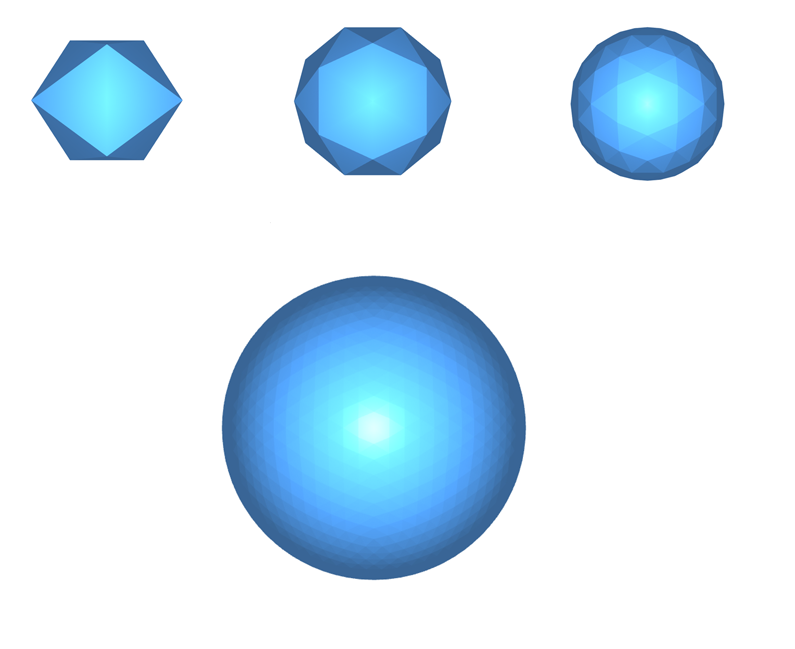
\includegraphics[scale=0.24]{./images/icospheres/icosphereslod.png}
\caption{Icosphere after different levels of iteration produced by our implementation. As mentioned it is clear that this system lends itself nicely for LODs systems}
\label{fig_isa}
\end{figure}

\begin{figure}
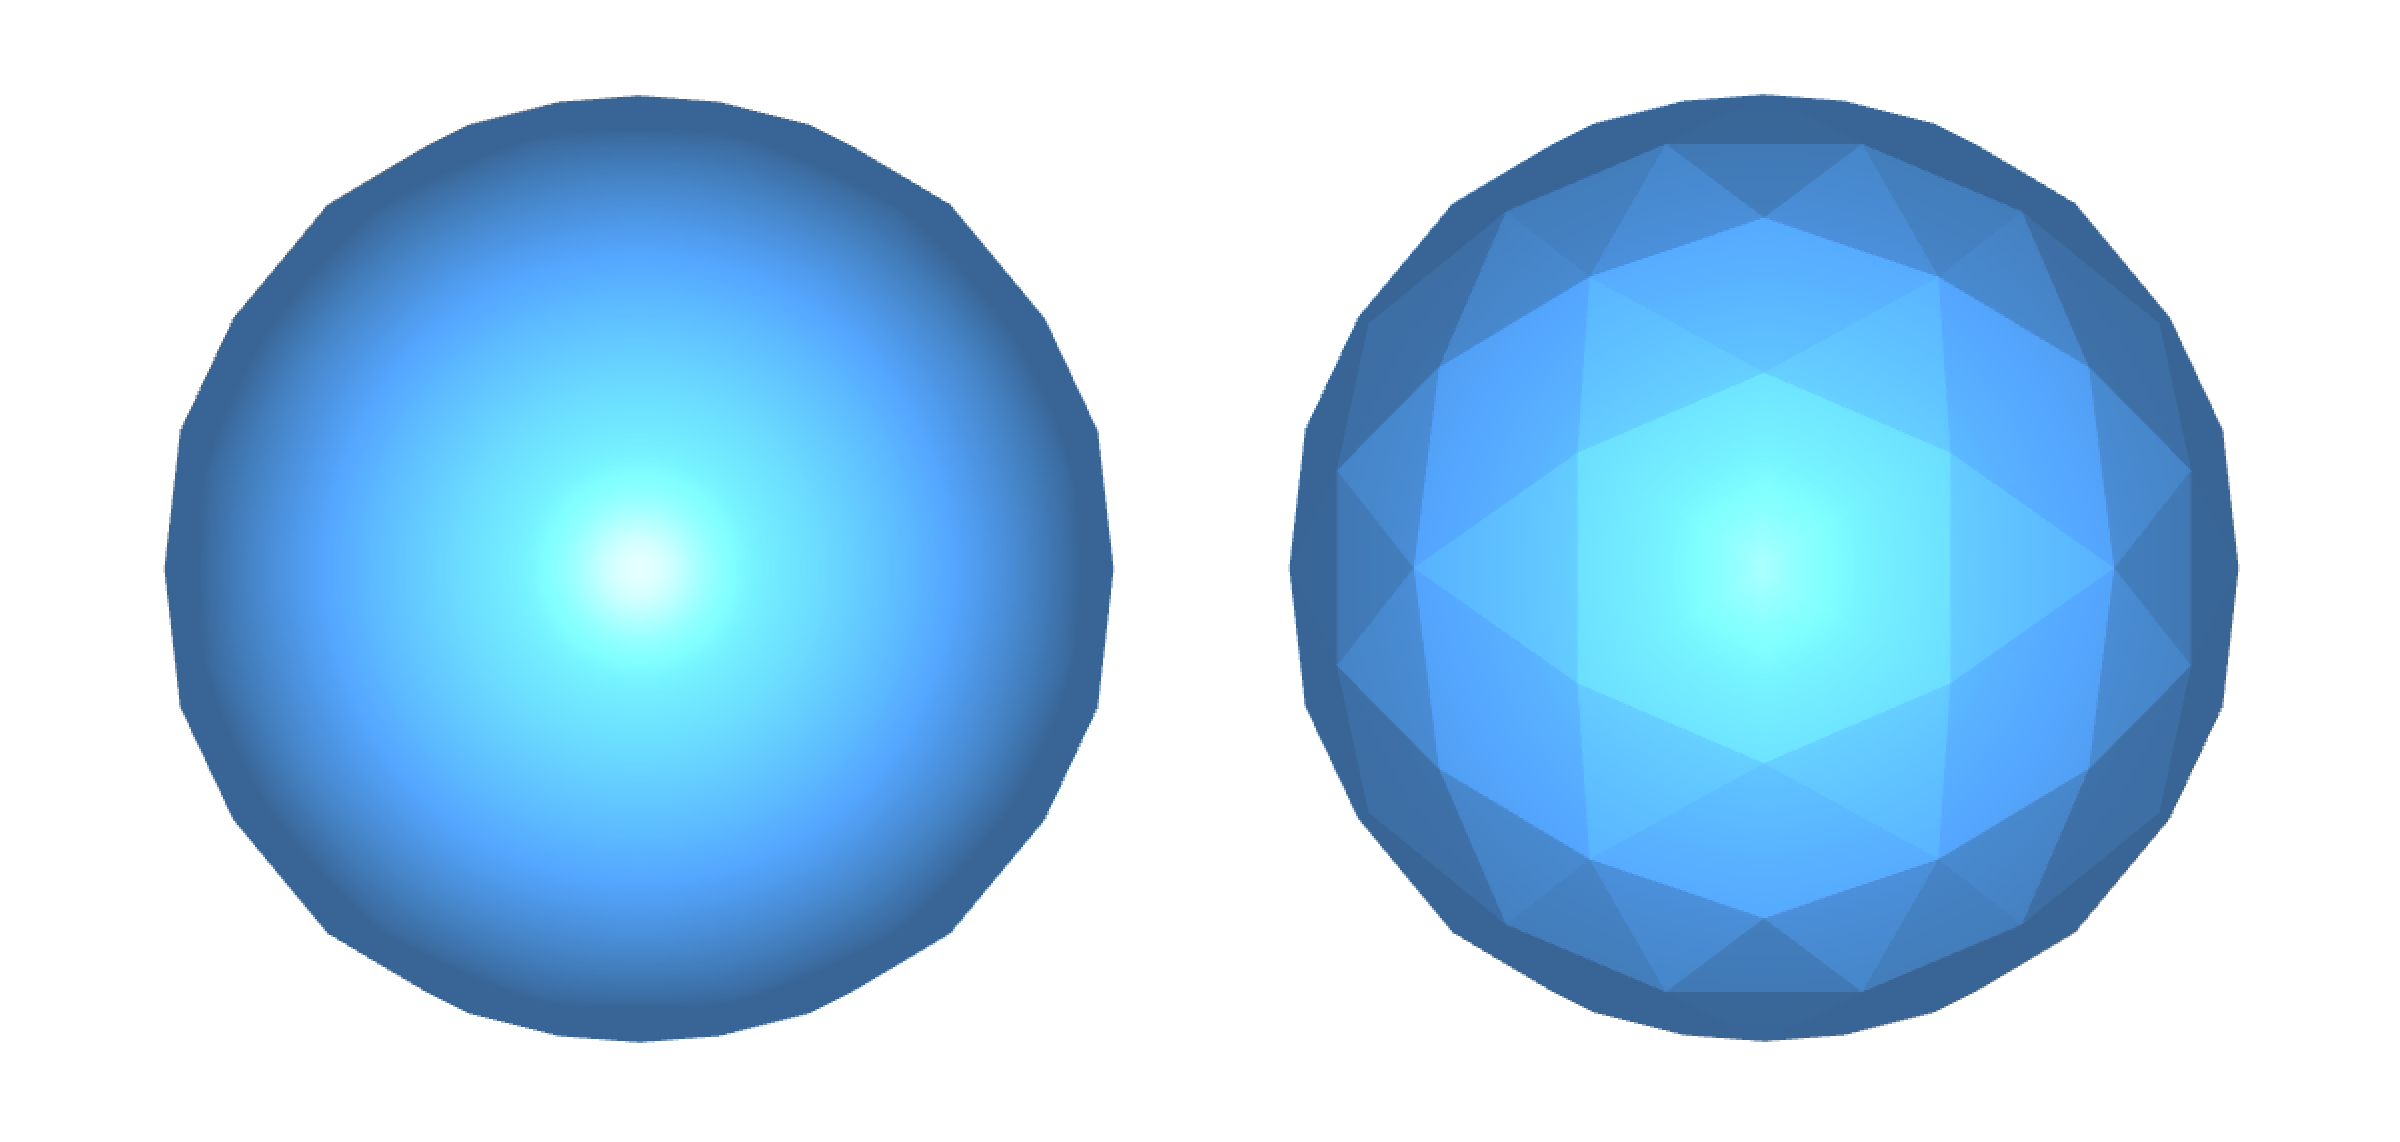
\includegraphics[scale=0.24]{./images/icospheres/icospheresnormals.png}
\caption{Left, the unmodified algorithm after 2 iterations that produces indexed meshes and interpolates vertex normals. Right, our modified algorithm that produces surface normals.}
\label{fig_isn}
\end{figure}

\section{\uppercase{Perlin Noise}}
\label{sec:pnoise}
\noindent Ken Perlin's algorithm for creating pseudo-random noise is a staple in any application trying to replicate natural occurring patterns. The algorithm is fairly simple and consists of three steps: defining an n-dimensional grid, computing the dot value of distance-gradient vectors and interpolating this values.

The process to create the noise is then repeated and the generation function is scaled, we call the scaled results octaves. Stacking these octaves gives the irregularity and details on different heights usually seen only naturally occurring phenomena. 

\begin{figure}
\centering
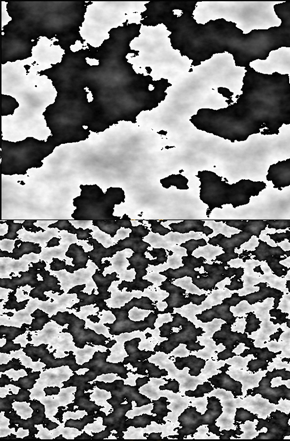
\includegraphics[scale=0.5]{./images/perlin_noise/combined.png}
\caption{Textures generated by our implementation of the Perlin Noise function.}
\label{fig_pn}
\end{figure}

\subsection{Multi Fractal Perlin Noise}
\label{sec:mfpnois}
Classical Perlin noise is homogeneous and isotropic, this plays against the rationale to use Perlin noise: creating natural occurring patterns.  As defined in \cite{ondrej07} a \textit{multifractal} is a heterogeneous fractal, this is achieved by parameterizing the dimension of the fractal function with another attribute, such as the height value of the terrain, this makes it so values closer to 0 (sea level) are smoothed out, whereas high values higher octaves have a bigger effect causing jags.  The algorithm implementation is based on \cite{pnoise} and [REF].

\section{\uppercase{Terrain Generation}}
\label{sec:tgeneration}

\noindent Using an instance of the multi-fractal Perlin noise, we deform vertexes as they are being created by the icosphere algorithm to create geographic-looking features. We use a \textit{ridged} version of the algorithm to produce more interesting patterns as described in [REF]. The terrain generation code can further parameterize the deformation by scaling the result or 

The deformation is the result of displacing the vertex by a value up to a maximum deformation in the direction of the vertex normal vector, which could be interpreted as 'up' in the terrains frame of reference, thus creating a relief.

Planetary terrain is colored per-vertex using a weighted color look-up table where the index is calculated using the vertex's 'altitude' (simply the magnitude of the vertex's position). The vertex colors are interpolated by the GPU and then applied per-pixel rather than using a texture.

\begin{figure}
\centering
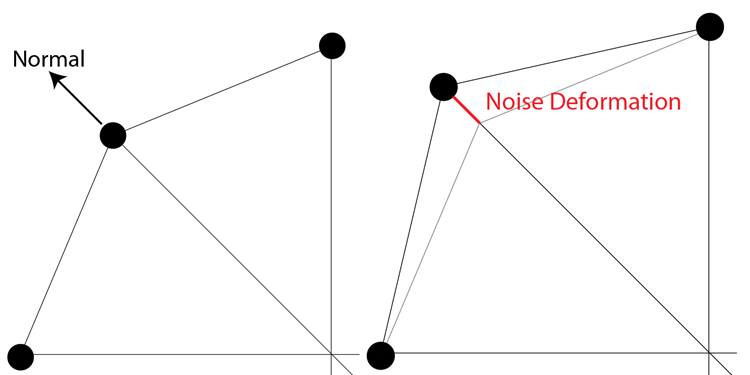
\includegraphics[scale=0.25]{./images/normals_deformation.png}
\caption{Terrain deformation illustrated}
\label{fig_tda}
\end{figure}

\begin{figure}
\centering
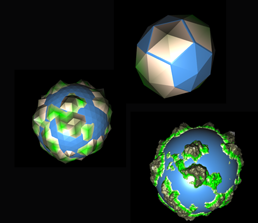
\includegraphics[scale=0.75]{./images/planets/planets.png}
\caption{The same planet at different levels of recursion.}
\label{fig_iterations}
\end{figure}

\section{\uppercase{Foliage}}
\label{sec:fol}
\noindent When planning the design of our foliage system, we initially look at using an L-System for the generation of trees, however due to our low polygon style, the detail that an L-System provides  was not needed, however we did use similar concepts for creating the tree branching. 
For the regular tree types there are three options or 'levels' that we can pass in as a parameter allowing for different tree variations. Figure \ref{fig_all_trees} and Figure \ref{fig_all_trees} show examples of the levels of branching, although our scene does not use Figure \ref{fig_all_trees}, this is just an example of how the basic concept of an L-System was integrated into our project.

Different types of tree assets were generated with similar algorithms, inclusive reusing some of the icosphere generation algorithm to create geometry. Figure \ref{fig_all_trees} shows examples of different trees generated by our system.

\begin{figure}
\centering
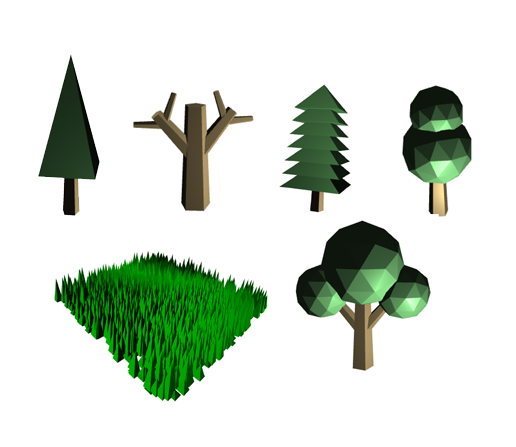
\includegraphics[scale=0.3]{./images/trees/alltrees.png}
\caption{Different types of vegetation generated by the system.}
\label{fig_all_trees}
\end{figure}

\bibliographystyle{apalike}
{\small
\bibliography{tinyplanets}}
\vfill
\end{document}

